The WR technology \cite{Wlostowski2011} is an international collaborative
project started at CERN in 2009, later joined by other worldwide laboratories and
companies. It was born as a replacement technology for CERN's accelerator timing system,
but due to its versatility and improved performance compared to other
alternatives, together with its open nature, it was quickly adopted by other
scientific institutions. \textcolor{red}{There is also a strong interest amongst private companies to
extend WR to the industrial domain, such as Seven Solutions S.L. 
\cite{sevensols:wr} [esta frase, en mi opinion, es un canteo]} 
\textcolor{teal}{Cierto, pero a mi tambien me gusta hacer el guigno a seven en 
los papers. Yo daria fuerza a la frase para obligar a referenciar a seven. Como 
dices que hay un fuerte interes (que realmente es mentira porque si no seven no 
tendria nada que hacer... ) da algunas muestras de ese supuesto interes: cuando 
dices lo del industrial domain da tres ejemplos como gps backup, smart grid y 
cualquier otra mierda, haces link a la pagina de proyectos de 7s que es 
realmente lo unico que hay y todos contentos}. 
Furthermore, from its very early stages, WR was launched as an open SW/HW
initiative with available online sources at CERN's Open Hardware Repository (OHWR)
\cite{ohwr:repo}. This encouraged different companies and research institutions
to openly collaborate in its development.

The WR protocol extends PTPv2 with extra messages and has been proposed to be
included in the new PTP release (PTPv3) as High Accuracy (HA) profile
\cite{wr:maciej-ptpv3-standard} . Its main goal is to provide a synchronisation
accuracy better than 1 ns and precision in the scale of ps. The major
improvements introduced by the WR protocol address weak aspects of the PTPv2:
the limitation of the phase difference measurements to one period of the system
clock; and the assumption of symmetry between transmission and reception
paths. It inherently performs self-calibration over optical fibre links and it
is capable of distributing time to a very large number of devices with very
small degradation. Nevertheless, this technology was not designed originally
to address synchronization over long distance links, neither the inclusion of monitoring and dependable
mechanisms on the nodes. Although SKA is working on improving both issues, this contribution
particularly presents a new platform capable of disseminating the PPS signal incorporating flexibility and dependability features.  
\gutinote{cuales son las dependability features?}

The WR synchronisation mechanisms include the following elements:

\begin{itemize} 
        \item {Frequency synchronisation (syntonization): It uses
		physical layer (L1) of Synchronous Ethernet (SyncE) 
		\textcolor{teal}{NOOOOOOO!!!! Si lo he leido antes y se me ha escapado 
		decirlo es para pegarme una paliza. Supongo que lo que pretendia leer 
		es que se recupera la señal de reloj con la que se codifican los datos 
		en la capa fisica o L1 del modelo OSI (sin mencionar a SyncE)} to encode
	    the clock signal in the data stream. } 
        
        \item {Phase synchronisation:
		Thanks to the syntonization, both nodes in a link are able to
		recover the other physical clock and compare it to its own clock
		in order to get the phase difference. The phase measurement is
		performed by an IP core known as Digital Dual Mixed Time
		Difference (DDMTD) present in the gateware design.\textcolor{teal}{Yo 
		reescribiría el párrafo porque no queda claro por qué se necesita la 
		sintonización para el DDMTD (me acabo de encontrar esto: 
		http://www.ee.ucl.ac.uk/lcs/previous/LCS2011/LCS1136.pdf, quizás sea 
		interesante referenciarlo). Aunque si lo dejas asi muy poca gente se 
		dara cuenta del fallo...} 
    
        \item {Time synchronisation: It is implemented by an enhanced
			version of the PTPv2 protocol and provides a global
			notion of time to the entire network. WR also takes into
			account the asymmetries in the propagation time due to
			the utilisation of different wavelengths in the same
			fibre link improving the accuracy of standard PTP
			protocol.} \end{itemize}

WR implements mechanisms to ensure deterministic and reliable data transfer
between thousand of nodes connected over optical fibre links up to 10 km.
However, it can easily be extended up to 50 km without significant degradation
and up to 120 km without the needs of optical amplification 
\textcolor{red}{alguna REF de esto??} \textcolor{teal}{No creo que sea 
necesaria una ref si se comenta en la frase que se puede extender facilmente 
hasta 120 (nada de primero 50 y luego 120, eso es tonteria) utilizando modelos 
de sfps ya existentes en el mercado (es un producto que se compra no es 
ciencia, no hay misterio en pasar de enlaces de 10 a 120, solo dinero)}. 

\subsection{Network topology} \label{subsec:wr-net}

A typical WR network presents a tree topology and is composed of three different
kind of elements: a Grandmaster (GM), several intermediate devices such as
switches, and end-nodes as shown in the Figure \ref{fig:wr_hierarchy}. The GM
is normally connected to a very stable clock such as an atomic clock or a GPS
receiver \cite{Daniluk2012}. The intermediate levels of the network disseminate
the timing packets to the final nodes, which are composed of other devices such
as WR Switches, WR-ZENs or WR Light Embedded Nodes (WR-LEN) 
\textcolor{teal}{este si es un canteo de verdad, o mencionas una seleccion de 
nodos (donde no haya mas de uno de 7s) o nada}. These devices have
several ports and can behave as PTPv2 Boundary Clocks (BC). Moreover, they are
connected using the master-slave scheme: some ports act as slave (upstream)
of the to the upper layer while the others are masters (downstreams) and
they are in charge of propagating the synchronisation to the next level of the
hierarchy. The nodes of the last level of the network are known as slave devices.
They recover the clock reference from the link and synchronise their local
oscillators in order to provide a time reference for a specific application.

In addition to the conventional tree topology of the timing networks, new
network topologies are currently under-study in WR to add some mechanisms to improve fault
tolerance and security. Examples of this research are
\cite{jlgutierrez-paper-redundancy} and \cite{jlgutierrezhsr} that incorporate Transparent Clocks
(TC) and redundancy protocols to the WR technology such as
High-availability Seamless Redundancy (HSR) to ensure data delivery and reception in critical applications such as
control network, real-time applications or Smart Grids among others.

\begin{figure}[H] \centering 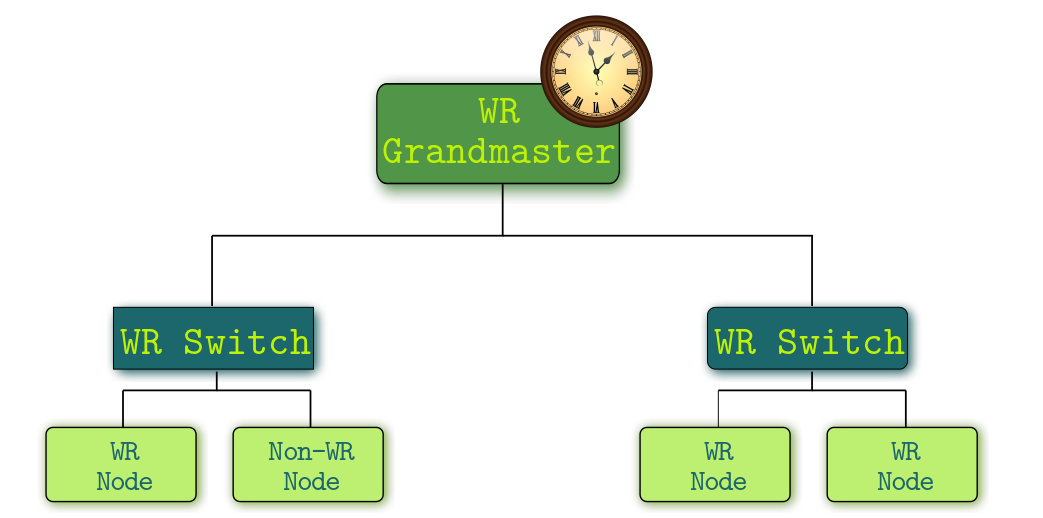
\includegraphics[scale=0.4]{img/wr_hierarchy}
	\caption{The WR network is a tree hierarchy where the root node is the
	GM that is responsible for distributing the reference time signals. The
	intermediate elements are WR Switches that acts as Gigabit Ethernet
	switchers \textcolor{teal}{Def. switcher: a person who administers 
	punishment by wielding a switch or whip, sobra algo no?} and as Boundary 
	clocks \textcolor{teal}{la puta o la f... los comentarios se me van de las 
	manos a ciertas horas. O se pone Boundary Clock (ambas con mayuscula) o 
	boundary clock (ambas con minuscula), pero no un mix} propagating the time 
	signals from the
	upper layers of the network. Finally, the main purpose of the end-nodes
	is to provide timing to another specific application.}
\label{fig:wr_hierarchy} \end{figure}

\subsection{WR devices survey for the SKA Telescope} \label{subsec:wr-dev}

Regardless of the case of use for the WR technology, it will be needed to select
a suitable set of WR devices. Most applications distinguish between two main roles
according to a typical WR network: devices which act as BC, and those that act as
Ordinary Clocks (OC). Currently, the WRS \cite{ohwr:wrs} is the most convenient
BC among all the WR devices. 

The WRS has a total of 18 Small Form-factor Pluggable (SFP) transceivers which 
\textcolor{teal}{seguro que es which y no where lo que pega aqui?? 
Fijate en que el sustantivo es one no which, por tanto aqui va una conjuncion 
no un pronombre.} 
one could be configured as slave
(upstream) and the rest as masters (downstream). It is also important to remark
another I/O ports such as: five coaxial RF connectors and one management
Ethernet RJ45 connector. Although there are other WR devices that could act as
BC, the WRS is the most appropriate for networks composed of a high number of nodes,
such as the SKA Telescope, because of its high number of SFP slots.

Nowadays, there  are several WR platforms that can act as OCs. 
For this reason, we have analysed three devices taking into account the specific requirements of the SKA project.

Table \ref{tab:wr_devcomp} contains a comparison between the following three WR
devices: \begin{itemize} \item The Simple PCIe FMC \textcolor{teal}{FMC no ha 
sido desglosado antes pero queda raro porque luego viene spec entre parétesis, 
que hacemos??} carrier (SPEC)
			\cite{ohwr:spec} is a WR-compliant FMC carrier that
			supports low pin count (LPC) boards. It includes a
			Xilinx's Spartan-6 FPGA, a SFP connector and a PCIe
			interface. It could be used in standalone mode
			\cite{migueljl-paper-wr-spec}, but due to its limited
			computational resources, the SPEC is usually used
			connected to a host PC using the PCIe interface.  No
			coaxial RF connectors are included in this board, being this fact
			a major penalty since a FMC board is required to retrieve the PPS signal.
	
	\item The WR Light Embedded Node (LEN) \cite{sevensols:wr_len} is a
		standalone WR node whose main design principles are: an easiness
		of use and a good timing performance. It was the first WR node
		that included the extended version of the WR PTP core (WRPC)
		architecture, the WR PTP Core Dual Port (WRC2P)
		\cite{torres2016scalability}. Besides the second WR-compliant
		Ethernet interface, the WR-LEN includes three coaxial RF
		connectors and a Ethernet RJ45 management port. Its design is
		quite similar to the SPEC board with some component
		upgrades, such as the FPGA (Xilinx's Artix-7). This device can act as BC and OC.
	
	\item The WR Zynq Embedded Node (ZEN) \cite{sevensols:wr_zen} is another
		standalone WR node but with many improvements compared to the
		rest of WR nodes. As in the WR-LEN, the WR implementation
		corresponds to the WRC2P.  This enables a BC configuration as
		well as OC, or GM configurations. Design is based on a Xilinx FPGA-SoC
		(Zynq-7000). It includes a dual ARM core included that enables the utilisation of a Linux-like
		OS. The board main I/O connectors are: a FMC high pin count
		(HPC), two SFPs, five coaxial RF and two Ethernet RJ45. The
		clocking resources include a low-noise oscillator and a flexible PLL schema.
\end{itemize}

 \begin{threeparttable}\centering \ra{1.1} \begin{tabular}{@{} lccc@{}}%\toprule
	 & \rotatebox[origin=c]{60}{SPEC} & \rotatebox[origin=c]{60}{WR-LEN}  &
	 \rotatebox[origin=c]{60}{WR-ZEN} \\ \midrule \textbf{WR-compliant}\\
	 \tab\small{+BC} & \Circle & \CIRCLE & \CIRCLE \\ \tab\small{+OC} &
	 \CIRCLE & \CIRCLE & \CIRCLE \\ \tab\small{+GM} & \LEFTcircle &
	 \LEFTcircle & \CIRCLE \\ \tab\small{+Standalone} & \LEFTcircle &
	 \CIRCLE & \CIRCLE \\
		
		\textbf{RF interfacing}\\ \tab\small{+PPS output} & \LEFTcircle
		& \CIRCLE & \CIRCLE \\ \tab\small{+RF I/O} & \Circle & \CIRCLE &
		\CIRCLE \\ \tab\small{+GM input} & \LEFTcircle & \LEFTcircle &
		\CIRCLE \\
		
		\textbf{Dev. support}\\ \tab\small{+Monitoring support} &
		\LEFTcircle & \LEFTcircle & \CIRCLE  \\ \tab\small{+Linux OS} &
		\Circle & \Circle & \CIRCLE \\ \tab\small{+Available resources}
		& \LEFTcircle & \Circle & \CIRCLE \\
		
		\textbf{Extensions}\\ \tab\small{+FMC connector} & \LEFTcircle &
 \Circle & \CIRCLE \\ \tab\small{+Redundancy} & \Circle & \LEFTcircle &
 \LEFTcircle \\ \bottomrule \end{tabular} \begin{tablenotes} \item \hfill
		 \small{\CIRCLE Fully supported; \LEFTcircle Partially
 supported; \Circle Not supported} \end{tablenotes} \caption{Comparison between
 three WR nodes.} \label{tab:wr_devcomp} \end{threeparttable}

Among other WR nodes, the WR-ZEN has been the chosen development platform for the
SKA Telescope PPS system due to its flexibility and main features. The possibility of being used as a standalone node
with Linux support, the inclusion of enough I/O ports (RF, FMC, etc.), together with an improved clocking resources
looks to fulfil the timing requirements of the project.

\textcolor{red}{falta nexo con la siguiente seccion}

%WR is designed to be fitted in a Field Programmable Gate Array (FPGA) device
%due to its flexibility to use in designs in a continuous development state.
%The source code is mainly written in Hardware Description Languages (HDLs) such
%as VHDL or Verilog. Moreover, there are several platforms that can implement WR
%that ensures the vendor-independent feature of WR. The most extended vendor in
%WR world is Xilinx, some examples of devices using Xilinx's FPGAs are the SPEC
%board \cite{ohwr:spec} and the WRS \cite{ohwr:wrs}. The other vendor used in WR
%is Altera. Some examples of boards could be found in \cite{cesar-altera-wr}.
%The main Intellectual Property (IP) block is the WR PTP core (WRPC) for WR
%nodes and the Real Time Subsystem (RTS) for WR switches. 

%The utilization of the previous WR-compliant nodes in the SKA system presents
%an important problem: they are based on PCIe interface cards to be plugged on
%standard computers, microTCA or VME-64 crates and therefore, a specific
%computer is necessary to provide the high level software management
%functionalities. Although most of these cards can be used on stand-alone
%operation mode, they just use a FPGA device as processing engine and this make
%very complicated to add new functionalities or standard software tools. The
%main WR node designs include a soft-microprocessor on the FPGA gateware but it
%is not enough to fully solve the problem because it requires using complex
%non-standard firmware programming tools and it normally translates on high
%time-intensive development effort and makes difficult the upgrade of the system
%firmware. We have worked with these platform in order to build a sensor network
%based on the SPEC board allowing the PC-hosted and the standalone modes
%\cite{migueljl-paper-wr-spec}.

%As a different solution, we present a new platform based on an enhanced
%technology: The WR Zynq Embedded Node (WR-ZEN) \cite{sevensols:wr_zen}. It is a
%new generation board that includes a Xilinx Zynq System-on-Chip (SoC)
%\cite{xilinx:zynq}. The Zynq SoC is composed of a FPGA and a hard ARM dual core
%microprocessor that can run an application that controls the hardware directly
%or a standard Operating System such as Linux that can host many different kind
%of processes at the same time. Moreover, the WR-ZEN allows developing gateware
%and software on the same chip, tightly integrating performance and flexibility
%thanks to the use of the co-design strategies. The WR-ZEN offers several
%advantages over the old WR-compliant nodes (WR-LEN, SPEC or SVEC) such as an
%enhanced standalone mode with a Linux system that can include high level
%software capabilities without an external PC and the new clocking circuitry
%among others. Accordingly, the WR-ZEN has been proposed to be used in the SKA
%project to implement the PPS distribution system and currently, it is being
%evaluated as a candidate solution for the SKA PPS distribution system.  

%Next sections will present the proposed system for SKA and the main WR
%contributions: WR Precision Time Protocol for clock propagation and the
%generation of PPS signal. 
